\documentclass{article}
\usepackage[utf8]{inputenc}
\usepackage[a4paper, total={6in, 10in}]{geometry}
\usepackage{titling}

\newcommand{\subtitle}[1]{%
  \posttitle{%
    \par\end{center}
    \begin{center}\large#1\end{center}
    \vskip0.5em}%
}

\title{Rhino/Grasshopper Plugin User Manual}
\subtitle{Esri}
\author{Aiulfi Loris}
\date{Version 0.5, October 2020}

\usepackage{natbib}
\usepackage{graphicx}
\usepackage{caption}
\usepackage{subcaption}
\usepackage{enumitem}
\usepackage{wrapfig}

\begin{document}

\begin{figure}
    \centering
    
\includegraphics[width=60mm]{res/rhino_plugin_base_icon.png}
\end{figure}

\maketitle

\paragraph{This document presents how to install and use the PRT Rhino command and Grasshopper components. This plugin allows to use the procedural runtime generation engine authored by Esri within Rhinoceros and Grasshopper.}

\tableofcontents

\section{Installation Instructions}

\begin{enumerate}
    \item Rhino 6 has to be installed in order for the plugin to work.
    \item In order for the plugin to be correctly loaded, it is needed to tick the "Ask to load disabled plug-ins" box located in Rhino's Tools $\rightarrow$ Options $\rightarrow$ Plug-ins.\\
    \begin{minipage}{\linewidth}
        \centering
        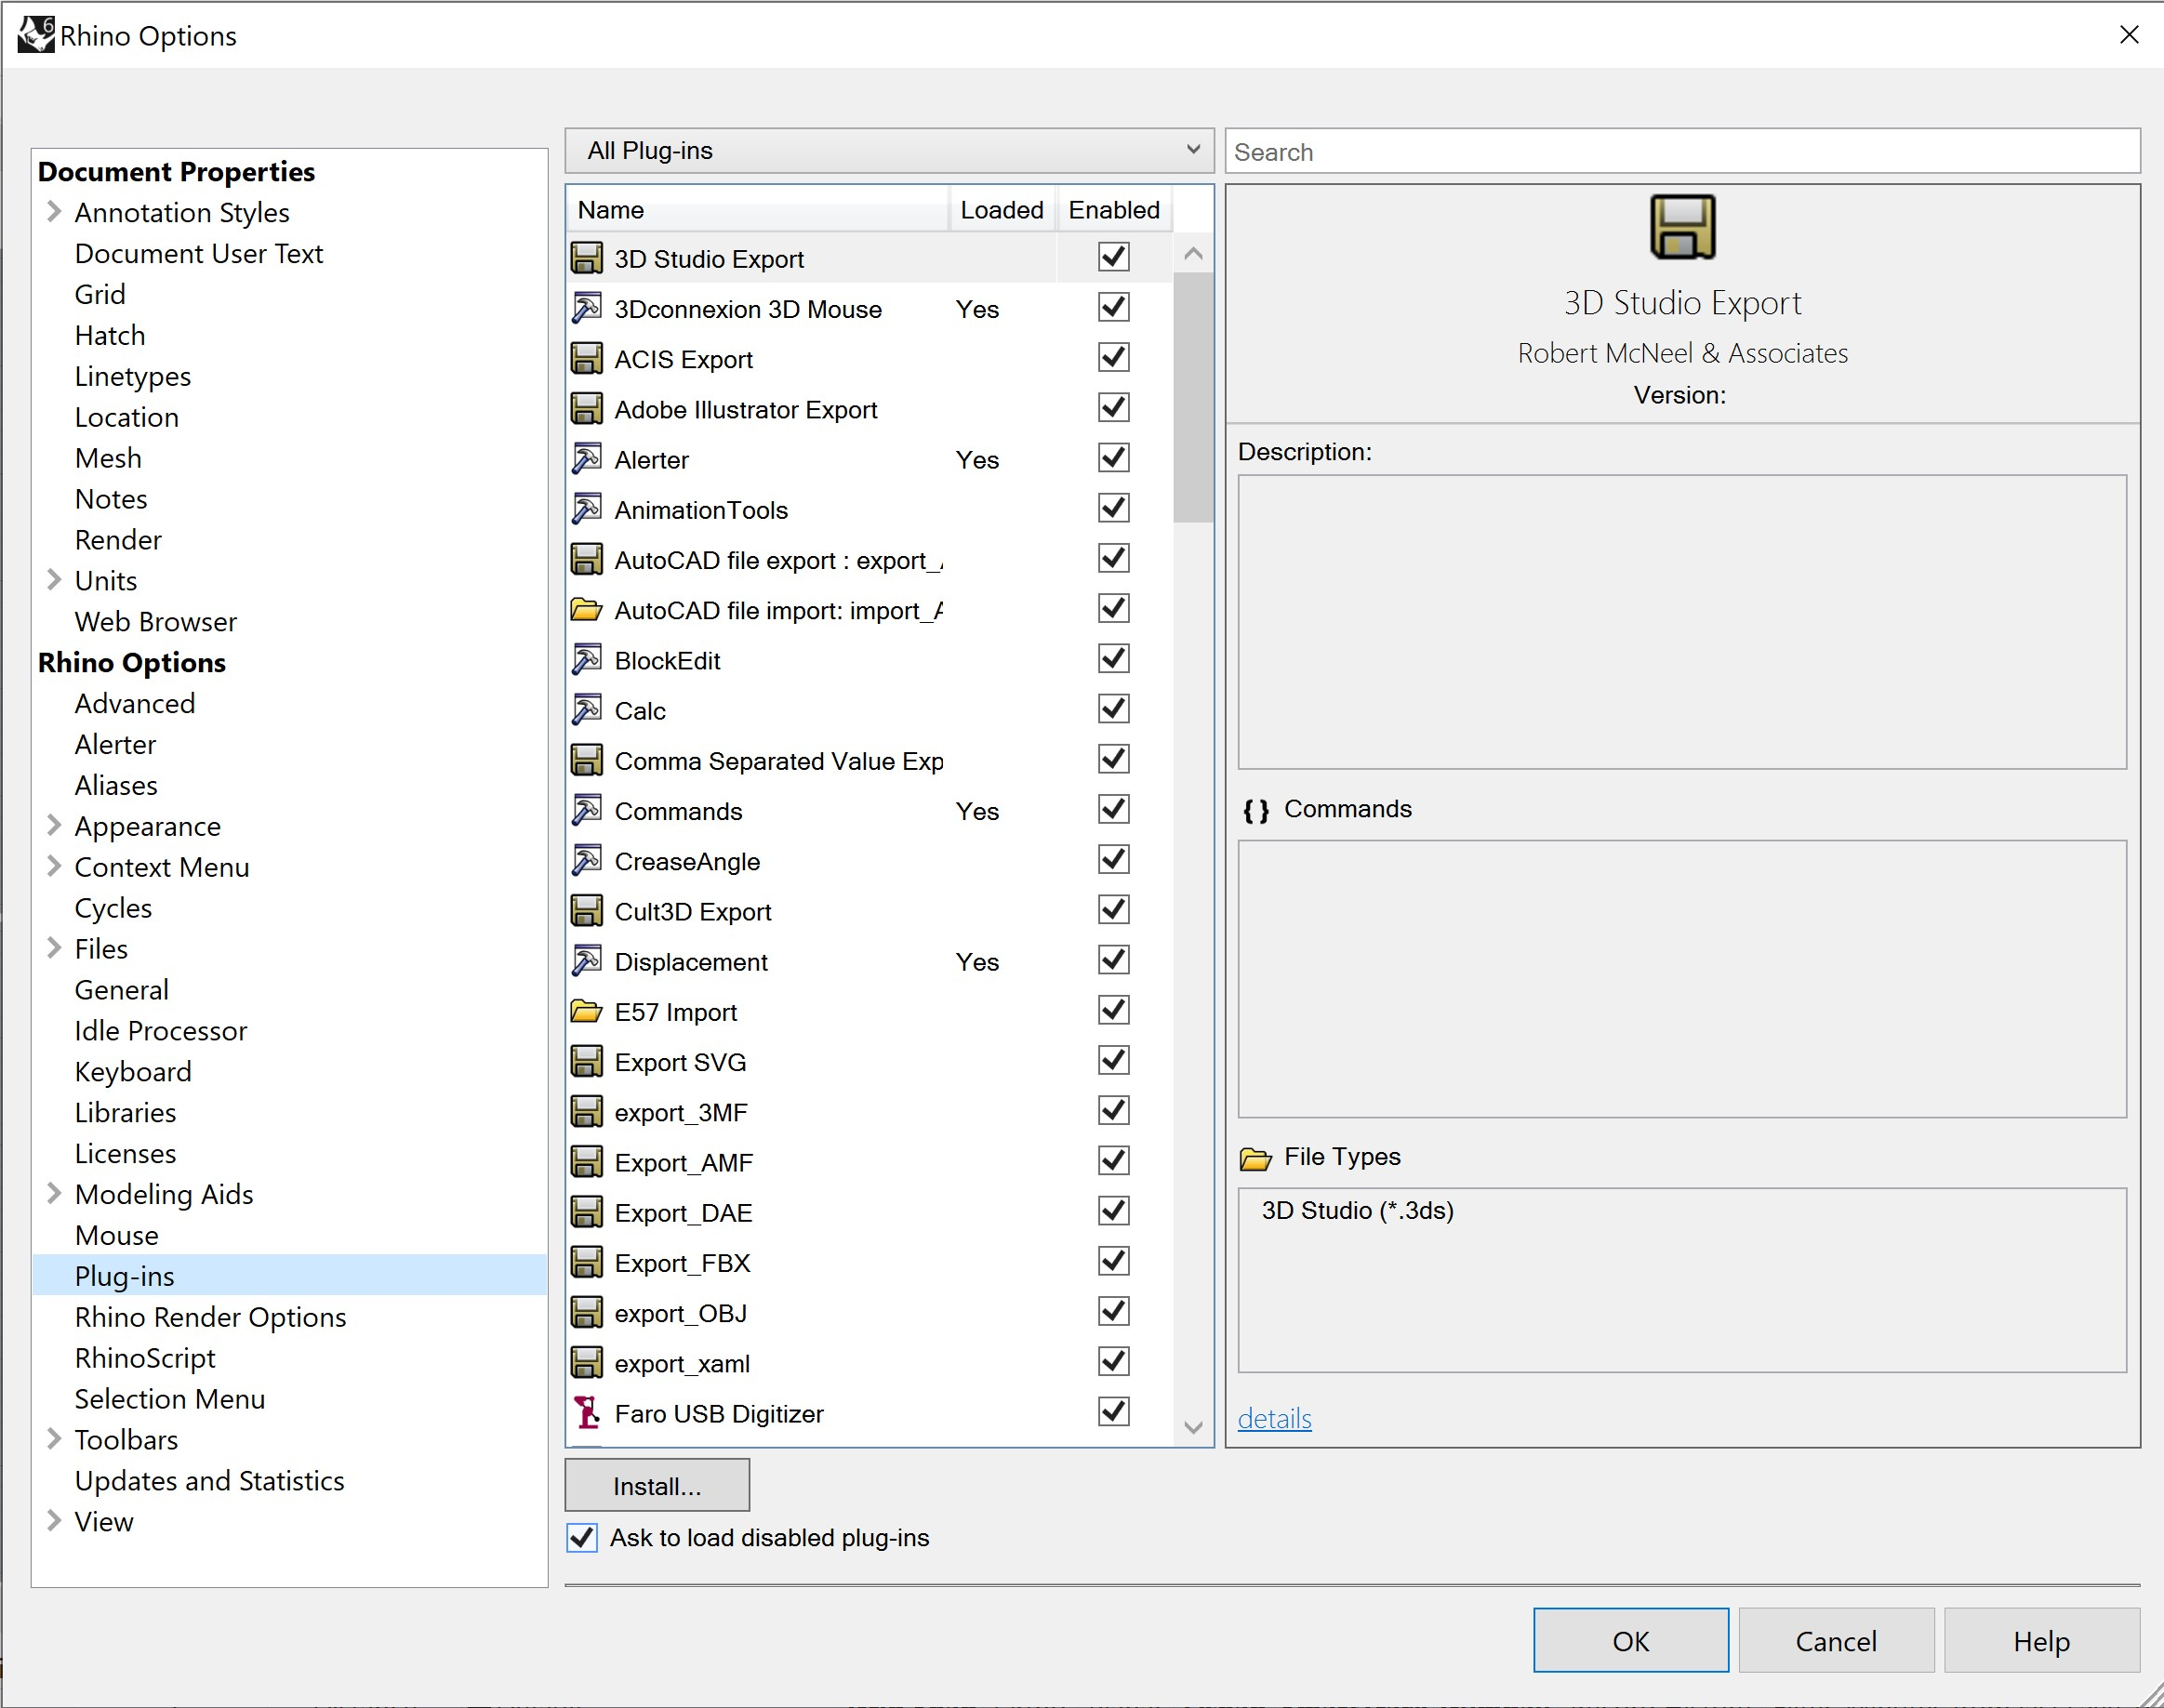
\includegraphics[width=10cm]{res/man_install_0}
        \captionof{figure}{Plug-ins option window.}
    \end{minipage}
    \item Close Rhino.
    \item Run the rhi package by double-clicking it.
    \item The package installer will open. Follow the instructions.\\
    \begin{minipage}{\linewidth}
        \centering
        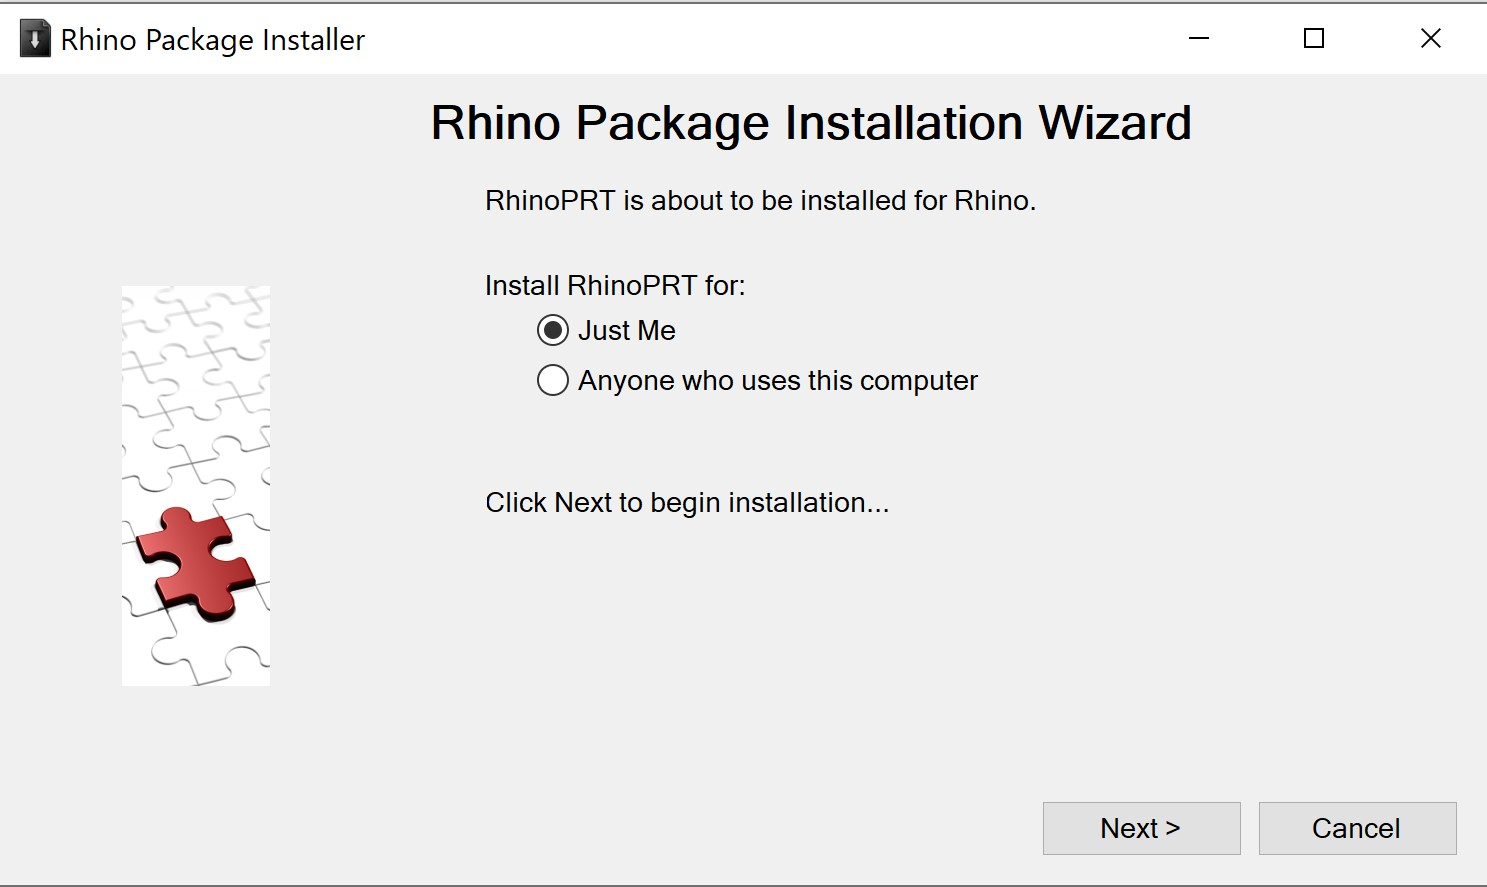
\includegraphics[width=10cm]{res/man_install_1.jpg}
        \vskip 0.5cm
        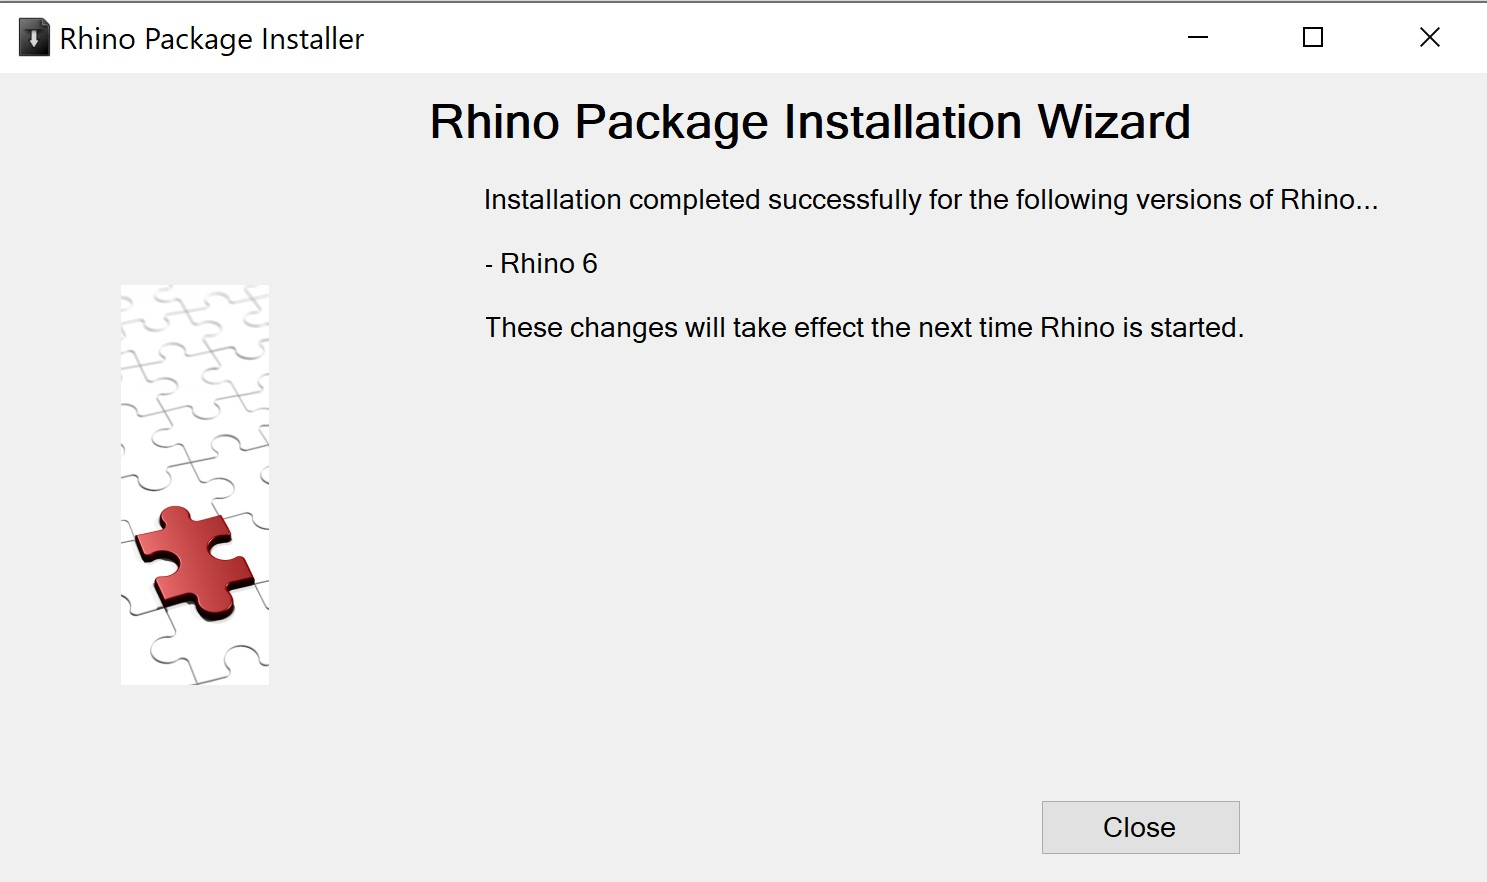
\includegraphics[width=10cm]{res/man_install_2.jpg}
        \captionof{figure}{Installation wizard.}
    \end{minipage}
    \item The plugin will be loaded at the next start of Rhino.
\end{enumerate}
\section{Rhino Command Usage}

\begin{enumerate}
    \item To start the Rhino plugin, run the command \textit{ApplyRulePackage}.\\
    \begin{minipage}{\linewidth}
        \centering
        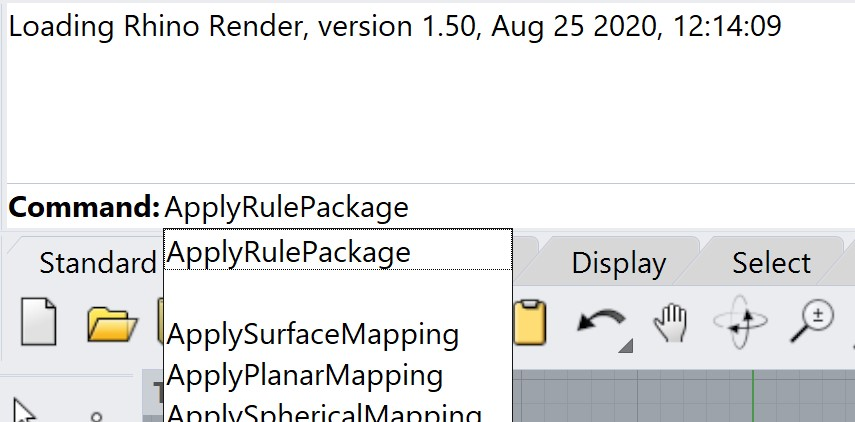
\includegraphics[width=10cm]{res/man_rhino_cmd}
        \captionof{figure}{The Rhino Command.}
    \end{minipage}
    \item It will open the file browser. Select a rule package (.rpk) and click open.\\
    \begin{minipage}{\linewidth}
        \centering
        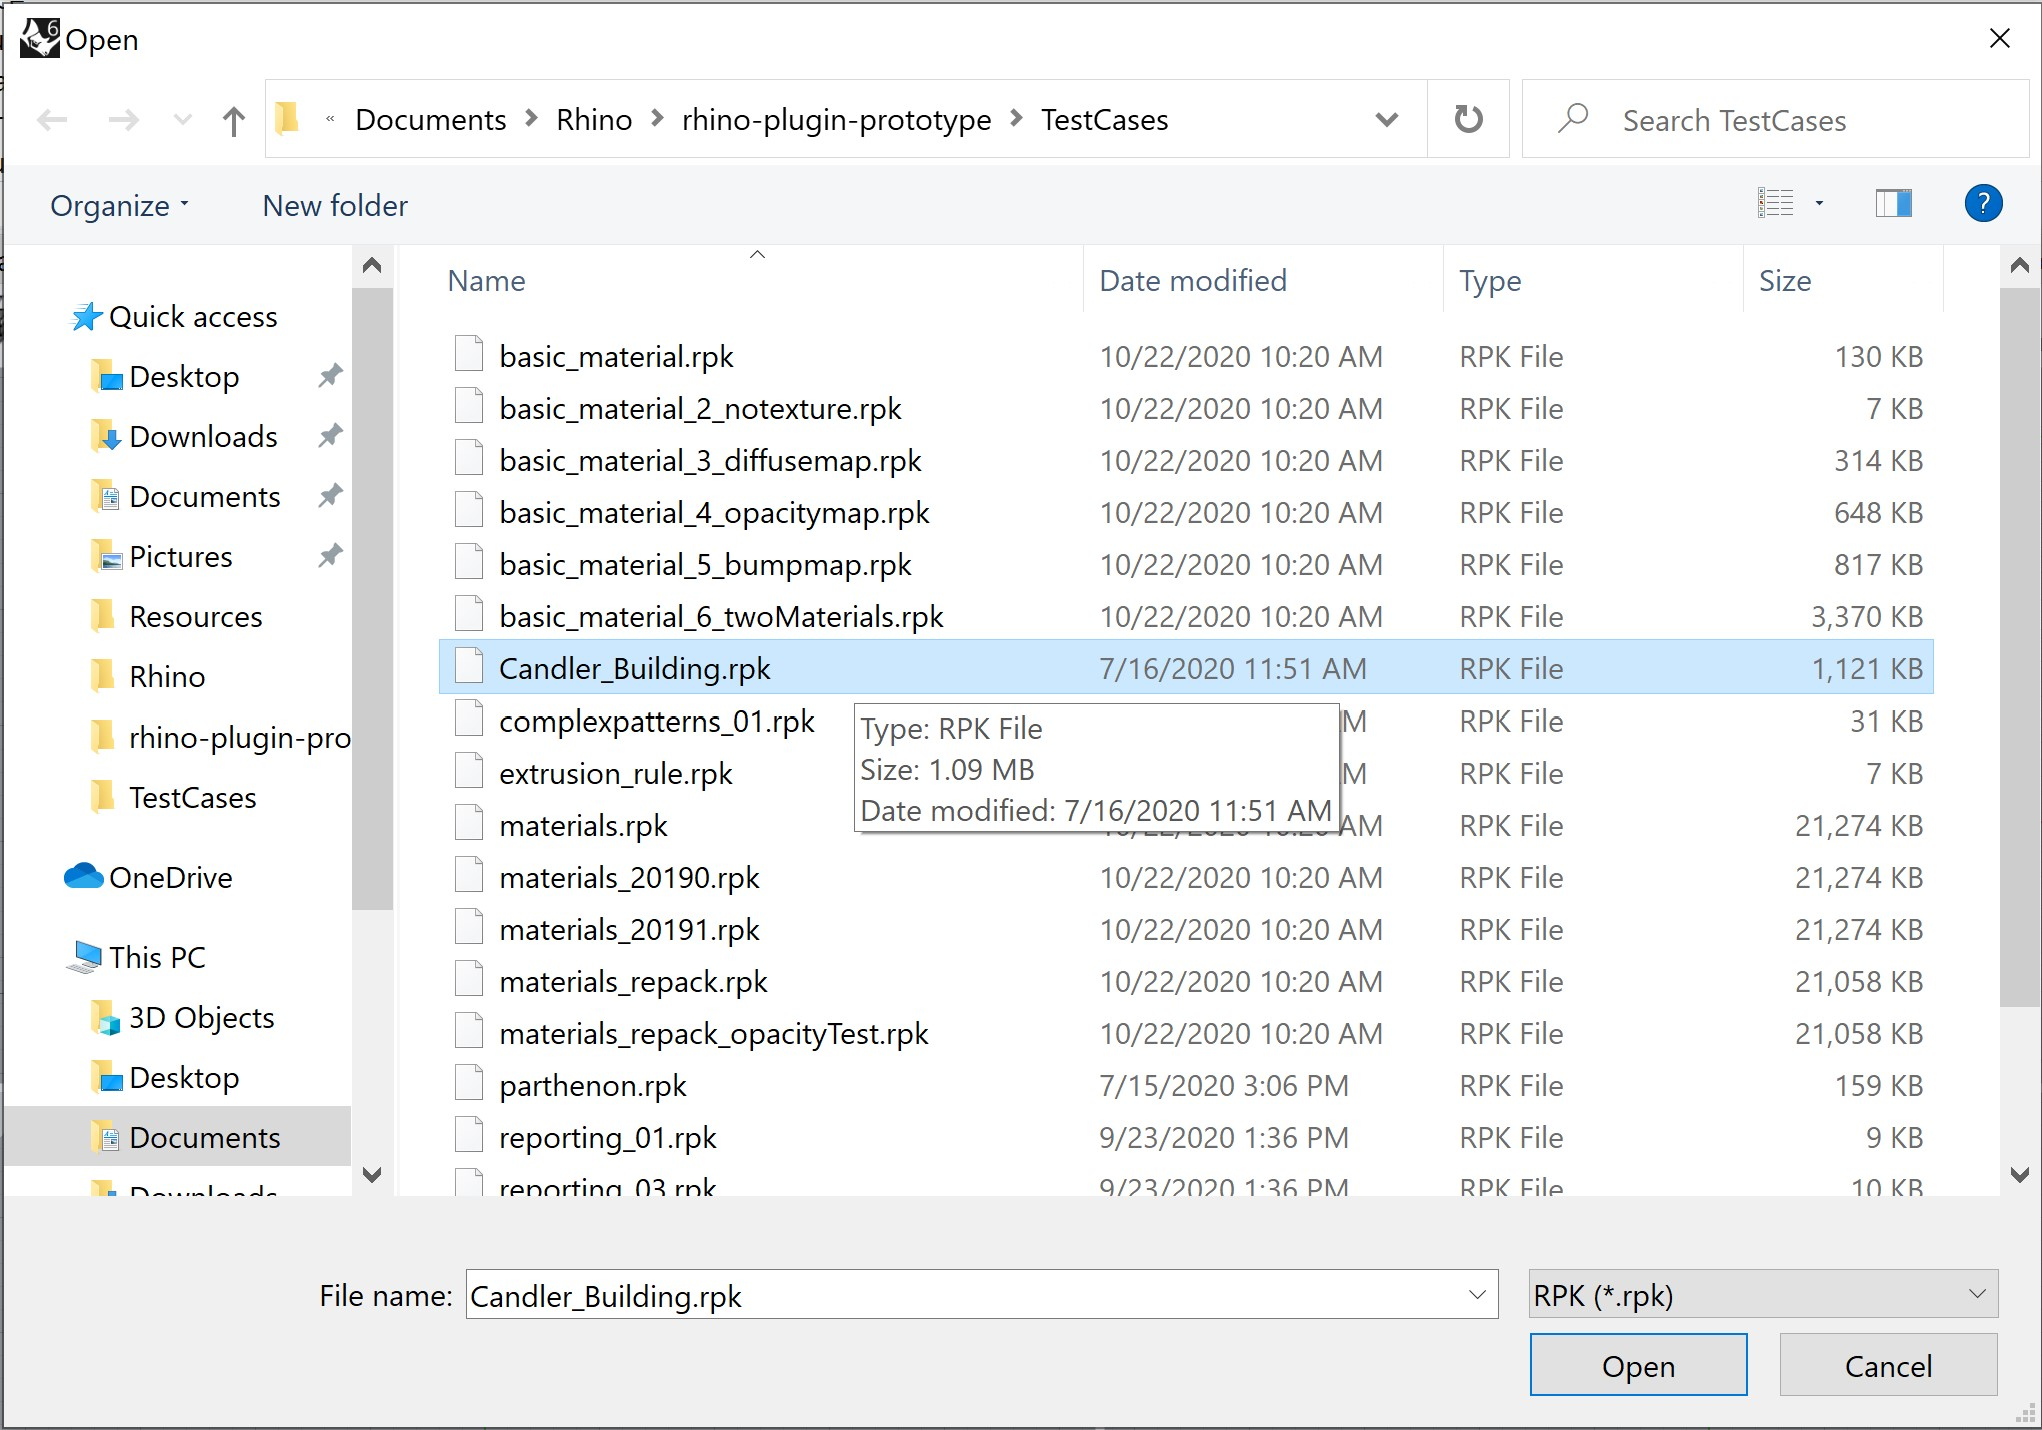
\includegraphics[width=10cm]{res/man_rhino_rpk_browser}
        \captionof{figure}{Choose a rule package.}
    \end{minipage}
    \newpage
    \item Select one or more starting shapes then press enter.\\
    \begin{minipage}{\linewidth}
        \centering
        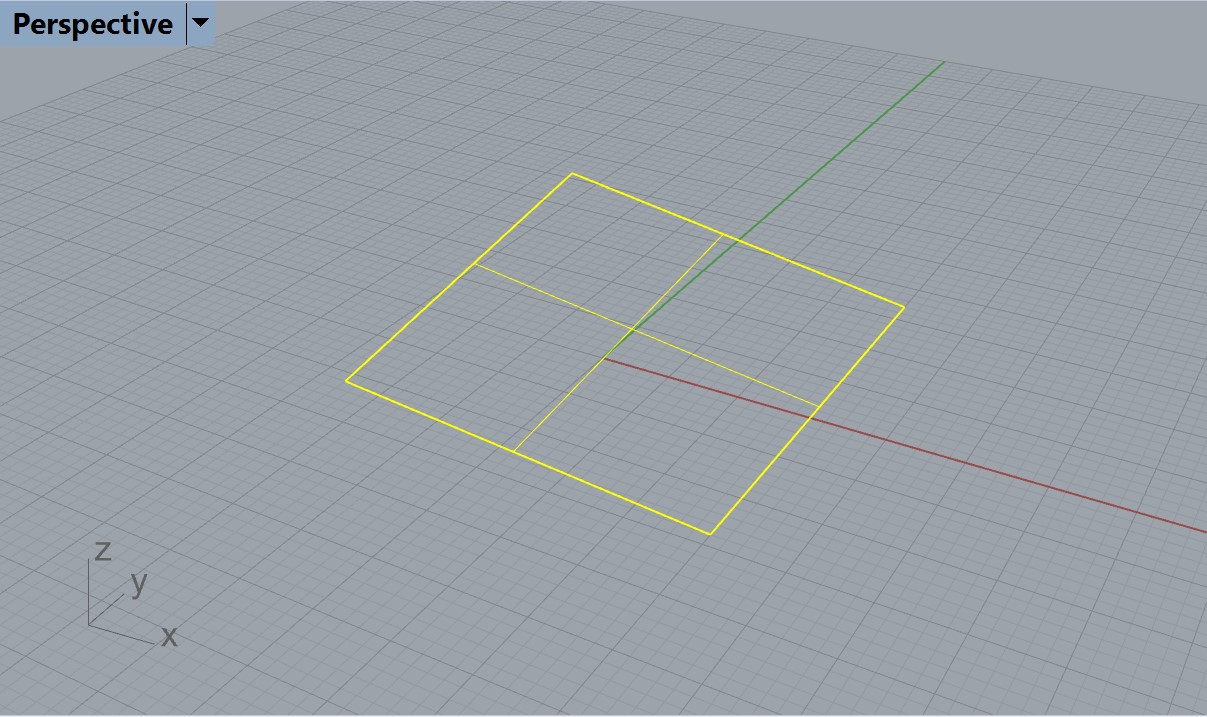
\includegraphics[width=9cm]{res/man_rhino_pick_shape}
        \captionof{figure}{Select one or more starting shapes.}
    \end{minipage}
    \item The resulting geometry will be generated and appear in the Rhino viewport.\\
    \begin{minipage}{\linewidth}
        \centering
        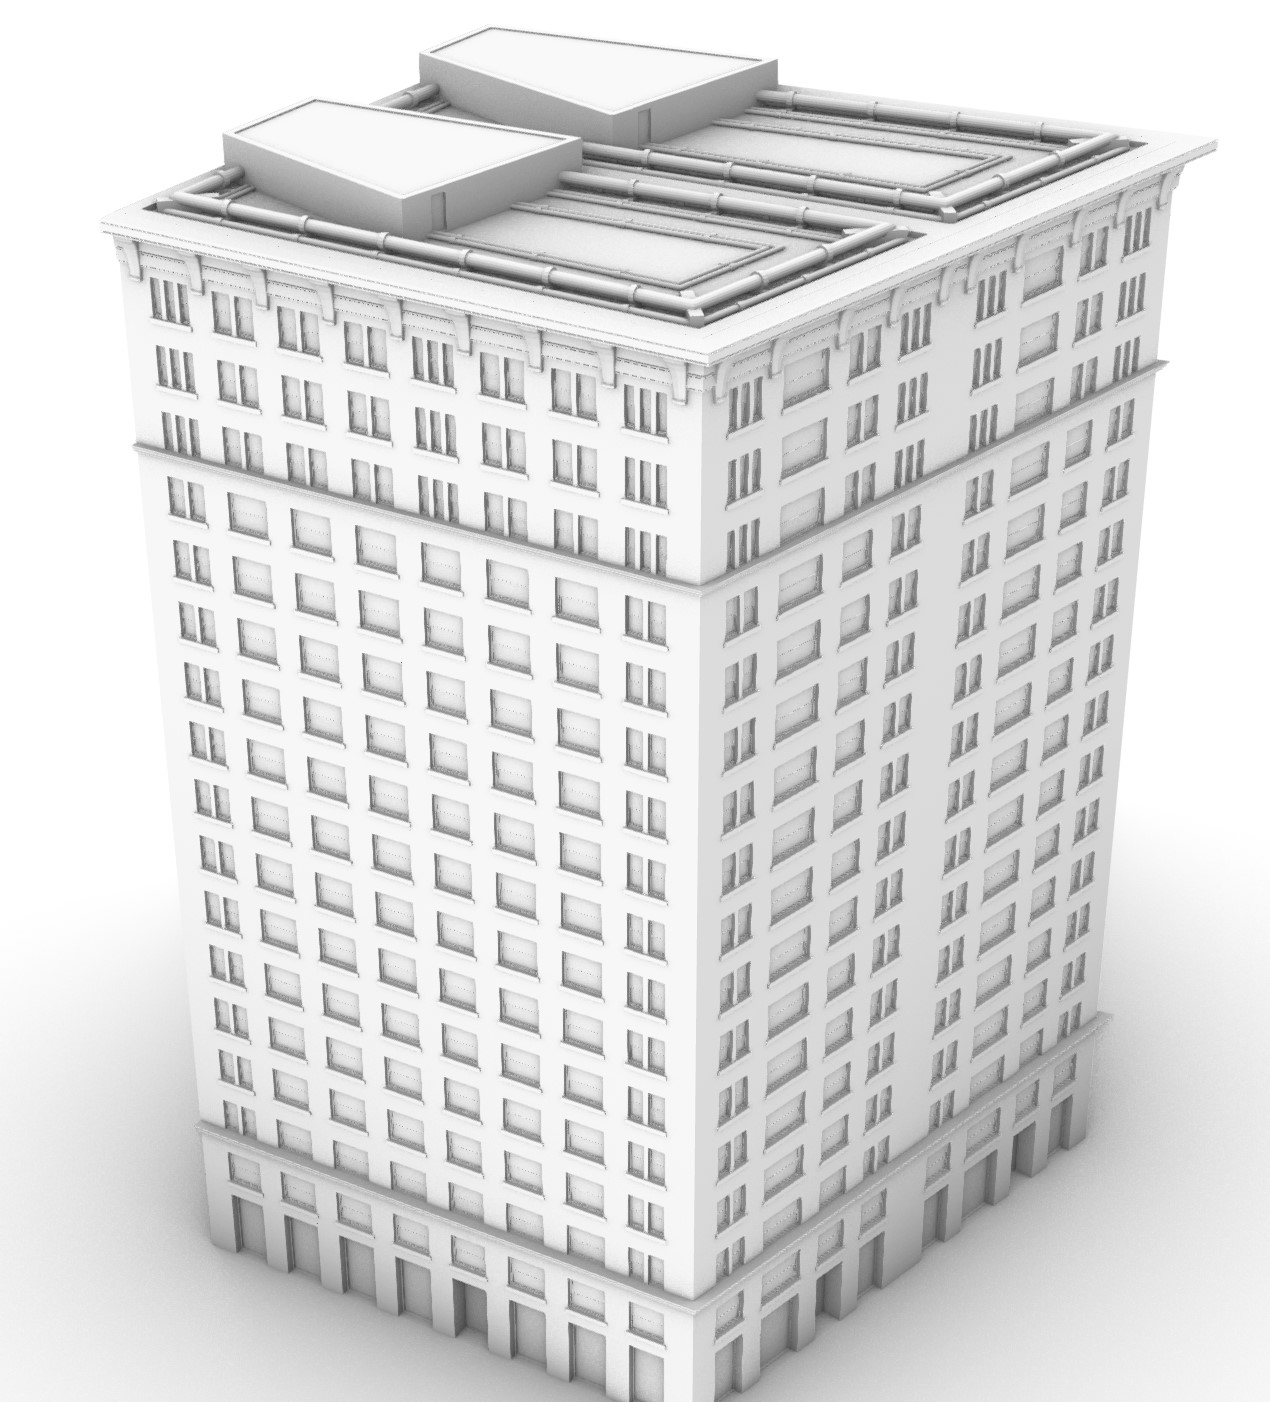
\includegraphics[width=9cm]{res/man_rhino_cmd_result}
        \captionof{figure}{Example of resulting geometry.}
    \end{minipage}
\end{enumerate}


\section{Grasshopper Components Usage}

Three components are added in a new tab named \textit{Esri}. The main one, whose purpose is to generate the shapes, materials and cga reports. The second one is used to preview and filter the cga reports. The third one is a simple helper component that unpacks the report into its three attributes. The components and corresponding icons can be seen in figure \ref{fig:gh_all}.

\newcommand{\subf}[2]{%
  {\small\begin{tabular}[t]{@{}c@{}}
   \mbox{}\\[-\ht\strutbox]
   #1\\#2
   \end{tabular}}%
}

\begin{figure}[h]
    \centering
    \caption{The grasshopper components}
    \label{fig:gh_all}
    \begin{tabular}{cc}
        \subf{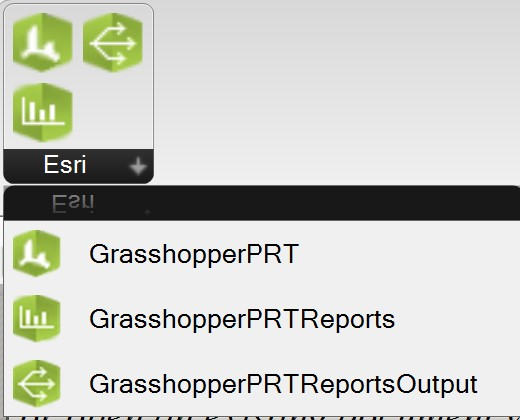
\includegraphics[width=42mm]{res/man_gh_icons.jpg}}{Icons of the components.}
        &
        \subf{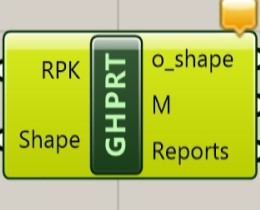
\includegraphics[width=52mm]{res/man_gh_main_comp.jpg}}{Main component.}
        \\
        \subf{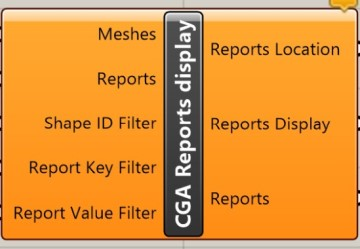
\includegraphics[width=60mm]{res/man_gh_filter_comp.jpg}}{Report filter and display component.}
        & 
        \subf{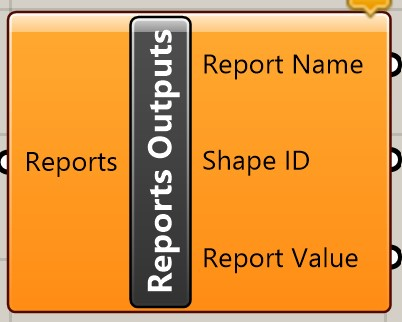
\includegraphics[width=52mm]{res/man_gh_unpack_comp.jpg}}{Report unpack component.}
    \end{tabular}

\end{figure}


\subsection{Main Component}

The main component takes two inputs by default (i.e. Fig \ref{fig:gh_main_input}). The path to a rule package (.rpk), can be provided by connecting a \textit{file path} component. The second input accepts various starting shapes. The list of compatible starting object is as follows:
\begin{itemize}
    \item $Mesh$
    \item $Rectangle$
    \item $Brep$
    \item $Surface$
\end{itemize}

\begin{figure}[h]
    \centering
    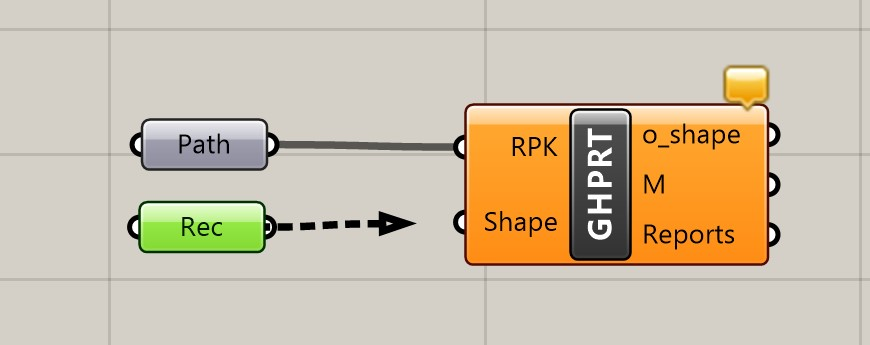
\includegraphics{res/man_gh_init_shape}
    \caption{Main component input parameters.}
    \label{fig:gh_main_input}
\end{figure}

Support for lines and points will be added in the future. When both default inputs are connected, the component is updated with rule attributes defined in the cga rules (Fig \ref{fig:gh_rule_attribs}). These rule attributes are added to the main component as input parameters. These parameters can then be connected normally with other components, or a value can be set directly by right-clicking on each parameter. Here is a list of currently supported input parameters and the corresponding component that can be connected to them:
\begin{itemize}
    \item Number (and array of numbers): \textit{number slider}
    \item Boolean (and array of booleans): \textit{Boolean}, \textit{Boolean Toggle}
    \item Text (and array of text): \textit{Panel}, \textit{Text}
    \item Colour (and array of colours): \textit{Colour}, \textit{Colour Picker} (Fig. \ref{fig:gh_color_picker})
\end{itemize}

\begin{figure}[h]
    \centering
    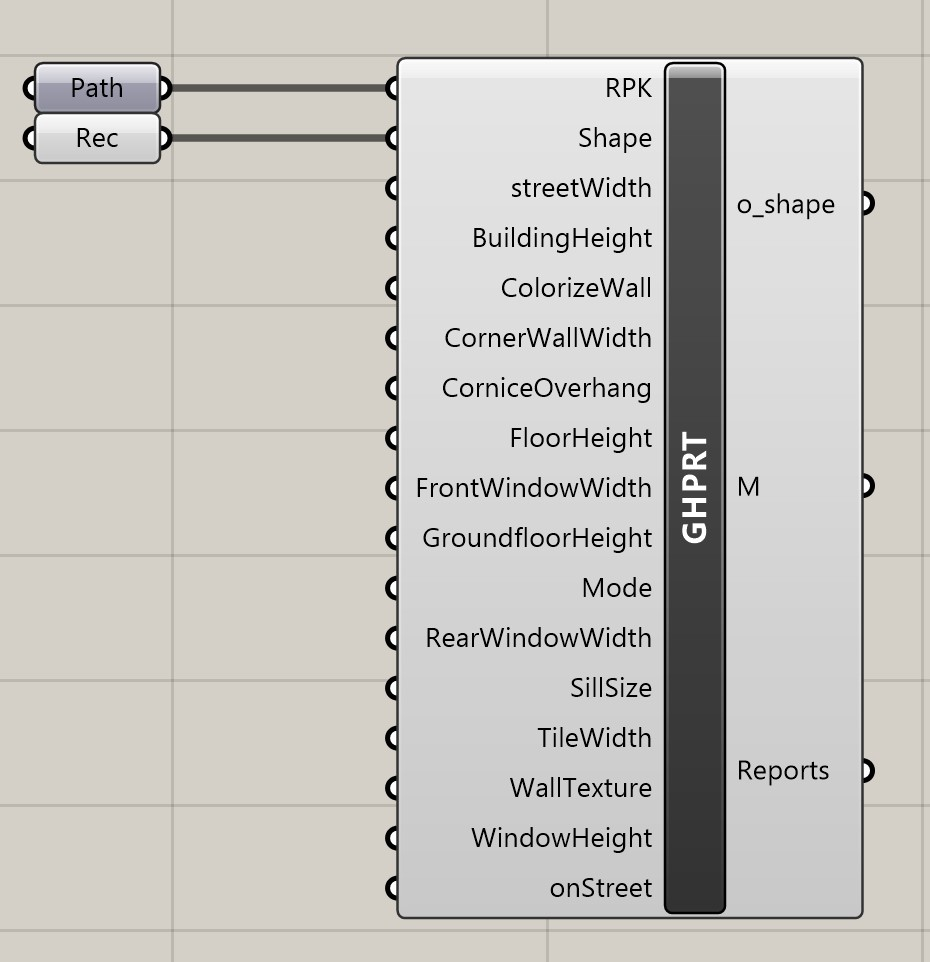
\includegraphics[width=60mm]{res/man_gh_rule_attributes}
    \caption{An example of component containing several rule attributes}
    \label{fig:gh_rule_attribs}
\end{figure}

\newpage

In order to gain more information on each rule attribute parameters, the user can hover with the mouse over each of them. A tool-tip is displayed, containing information on the expected data. Figure \ref{fig:gh_tooltips} shows two examples of such tool-tips. The first one is a number parameter that expects a number in the range from 28 to 150. The second example accepts a text parameter. The text can be chosen from a list of accepted choices listed in the tool-tip. Figure \ref{fig:gh_color_picker} shows the tool-tip of a colour attribute with a \textit{colour picker} component connected to it.

\begin{figure}[h]
    \centering
    \caption{An example of rule attribute tool-tips.}
    \label{fig:gh_tooltips}
    \begin{tabular}{cc}
        \subf{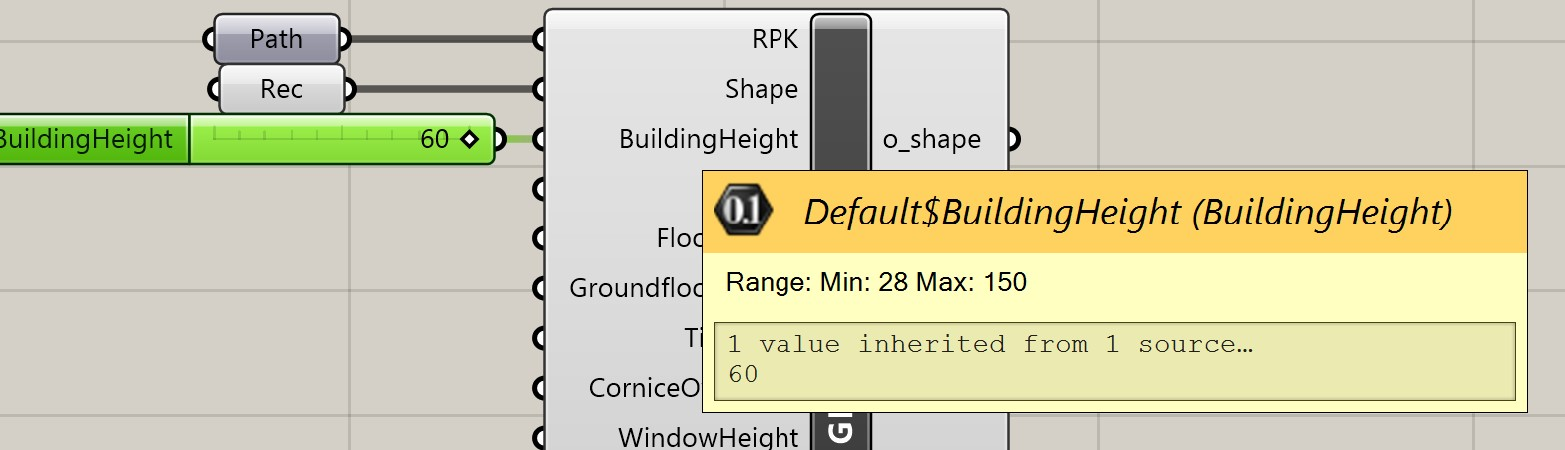
\includegraphics[width=60mm]{res/man_gh_input_tooltips.jpg}}{Tool-tip of a number parameter.}
        &
        \subf{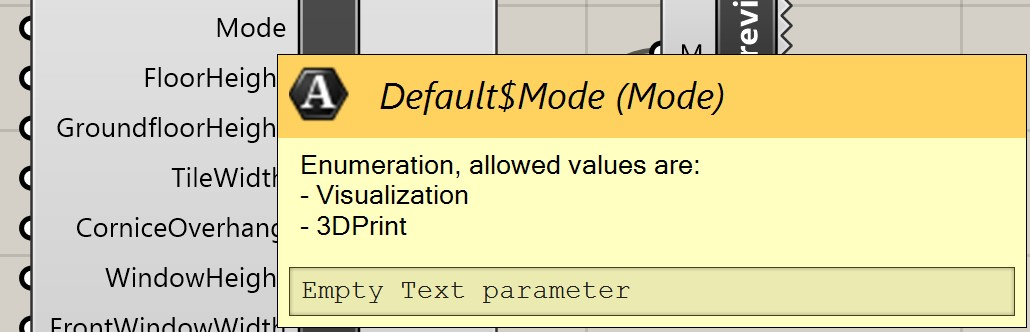
\includegraphics[width=60mm]{res/man_gh_enum_tooltip.jpg}}{Tool-tip of a text parameter accepting\\ list of defined strings.}
    \end{tabular}
\end{figure}
\begin{figure}[h]
    \centering
    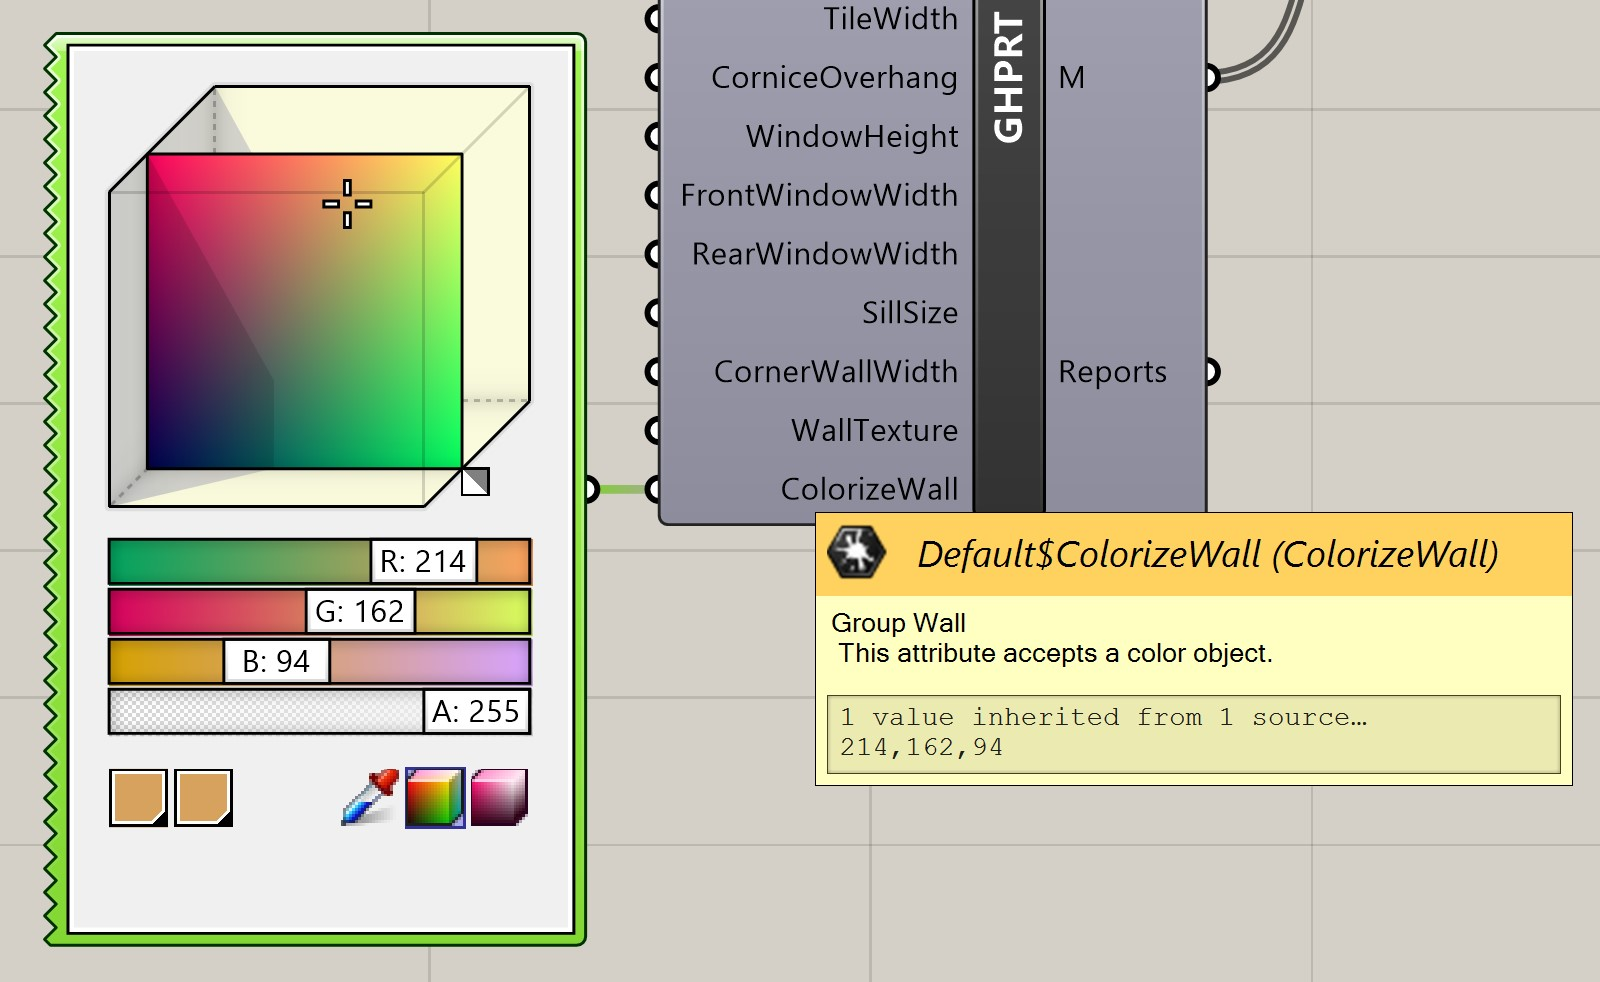
\includegraphics[width=60mm]{res/man_gh_color_input.jpg}
    \caption{The color picker component connected to a compatible parameter.}
    \label{fig:gh_color_picker}
\end{figure}

\paragraph{WARNING: There currently is an issue that prevents the tool-tips to be displayed before at least one of the input parameter is connected.}
\newpage

This component has three outputs:
\begin{enumerate}
    \item o$\_$shape: The generated meshes.
    \item M: The generated materials
    \item Reports: The generated cga reports.
\end{enumerate}

If materials are generated, they can be applied to the mesh by connecting a \textit{Custom Preview} Grasshopper component (Fig \ref{fig:gh_material}). The reports are outputted as a custom type. They are therefore not process-able by built-in Grasshopper components. To address this issue, two helper components are available. They are presented in the next two sections.

\begin{figure}[h]
    \centering
    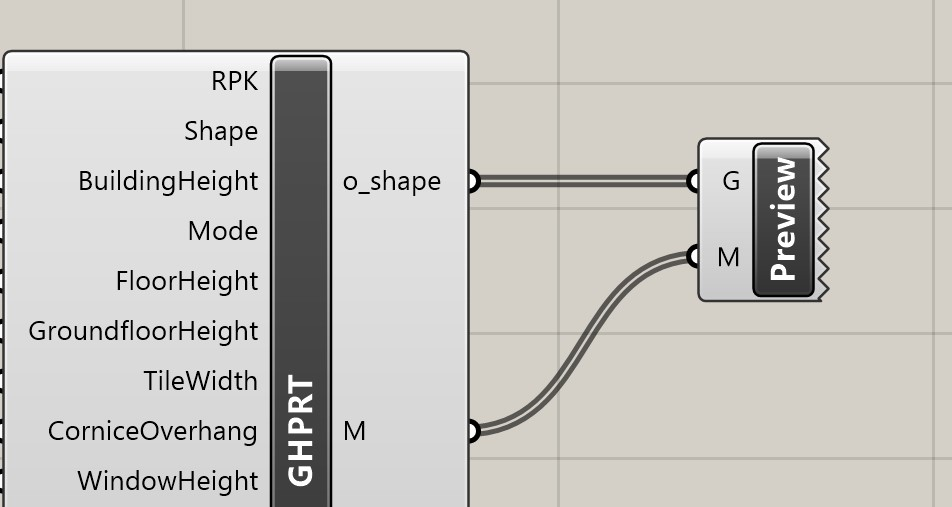
\includegraphics[width=60mm]{res/man_gh_apply_material}
    \caption{Use the custom preview component to apply materials.}
    \label{fig:gh_material}
\end{figure}

\subsection{Report Filter Component}

\begin{figure}[h]
    \centering
    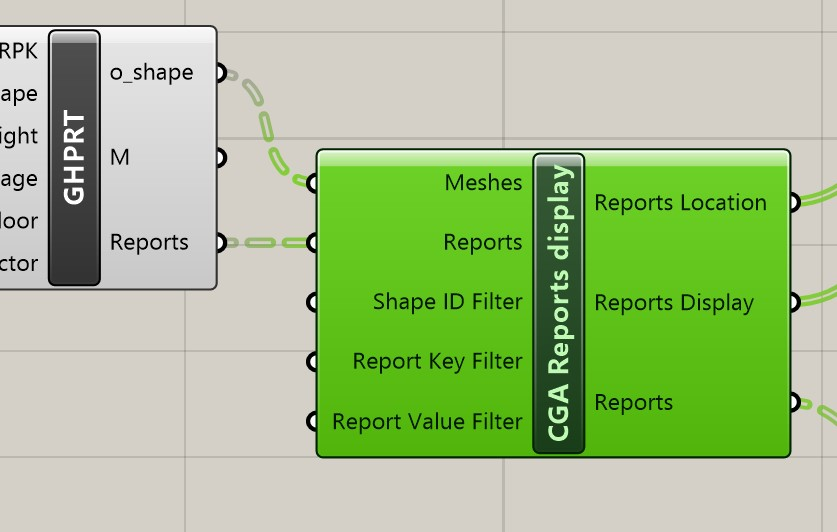
\includegraphics[width=60mm]{res/man_gh_filter_comp_connections.jpg}
    \caption{The report preview/filter component.}
    \label{fig:gh_filter_first}
\end{figure}

This component has 5 inputs. The first two can be connected to the main component's generated meshes and reports as shown in figure \ref{fig:gh_filter_first}. The next three inputs are optional filters:
\begin{enumerate}
    \item Shape ID Filter: Used to filter the reports by initial shape ID. Accepts a \textit{Domain} component.
    \item Report Key Filter: Filters the reports by name. Accepts a \textit{Panel} or \textit{Text} component, or a list of them. Report keys can be written on multiple lines.
   \begin{minipage}{\linewidth}
        \centering
        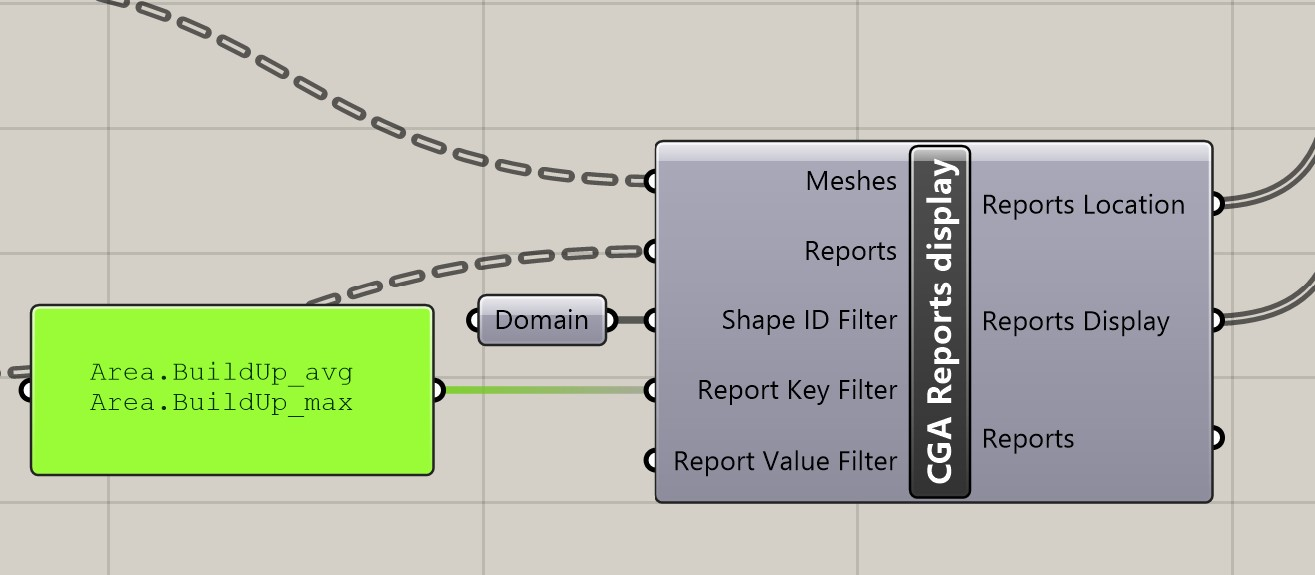
\includegraphics[width=10cm]{res/man_gh_filter_example.jpg}
        \captionof{figure}{Filter value usage.}
    \end{minipage}
    \item Report Value Filter: This input allows to select specific values for each keys selected in the second input.
\end{enumerate}

This component has three outputs, the first two can be connected to a \textit{3D Text Tag} component to display the selected reports in the Rhino view. The first one is simply a located plane used to correctly position and align the reports above each generated geometry. The second one provides the formatted reports, so they can be displayed. The third output simply provides the selected reports. These can then be unpacked by the component presented below.

\subsection{Report Unpack Component}

This helper component is very simple. Its task is to unpack the provided cga reports objects into primitive types that can be further processed by built-in Grasshopper components. It takes as input a list of report objects and outputs, for each report, its name (or key), the initial shape ID it belongs to, and the report value itself. Figure \ref{fig:gh_unpack_example} shows an example of such component.

\begin{figure}
    \centering
    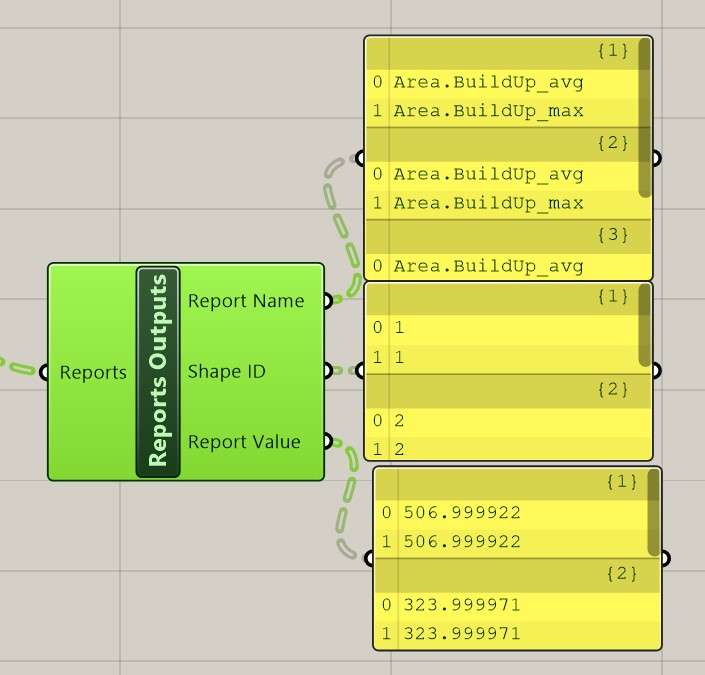
\includegraphics[width=60mm]{res/man_gh_report_unpack_connected.jpg}
    \caption{Report unpack component.}
    \label{fig:gh_unpack_example}
\end{figure}
\section{Known Issues}

\begin{itemize}
    \item Only the default style rule attributes are supported. Additional styles are currently ignored.
    \item A Grasshopper error is triggered when changing the rule package, if the new one has less rule attributes than the previous one. It does however not crash, just press \textit{OK} and the component will recompute correctly.\\
    \begin{minipage}{\linewidth}
        \centering
        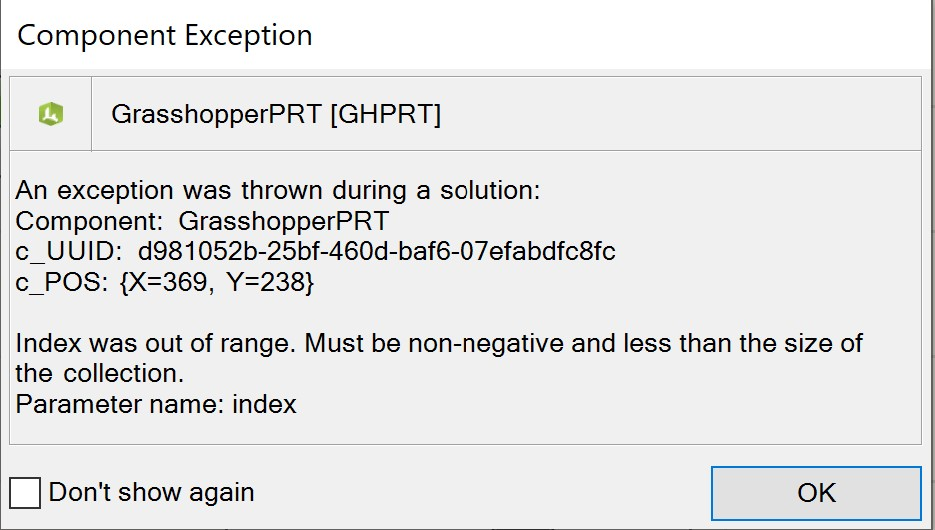
\includegraphics[width=9cm]{res/man_gh_error_1.jpg}
    \end{minipage}
\end{itemize}

\end{document}
